\section{Aufbau}
Zum Sammeln von Daten von Twitter verwenden wir einen Crawler, welcher über die Twitter-API Daten sammelt. Dazu ist es nötig diese Daten zu empfangen, dann zu puffern und schlussendlich in die Datenbank zu Schreiben. Allerdings müssen die Daten noch gefiltert werden, da wir nur Daten von verifizierten Twitter-Accounts (und manuell hinzugefügten) speichern. Sind die Daten gefiltert, werden sie vom Crawler noch lokalisiert. Das heißt, dass jedem Account beziehungsweise jedem Retweet eine Geoposition/Land zugeordnet wird. Ist dies erfolgt so werden die Daten in die Datenbank geschrieben.
\\ In \cref{fig:uml_crawler} ist der Aufbau des Crawlers anhand eines UML-Klassendiagramms spezifiziert.

\begin{figure}[h!]
	\centering
	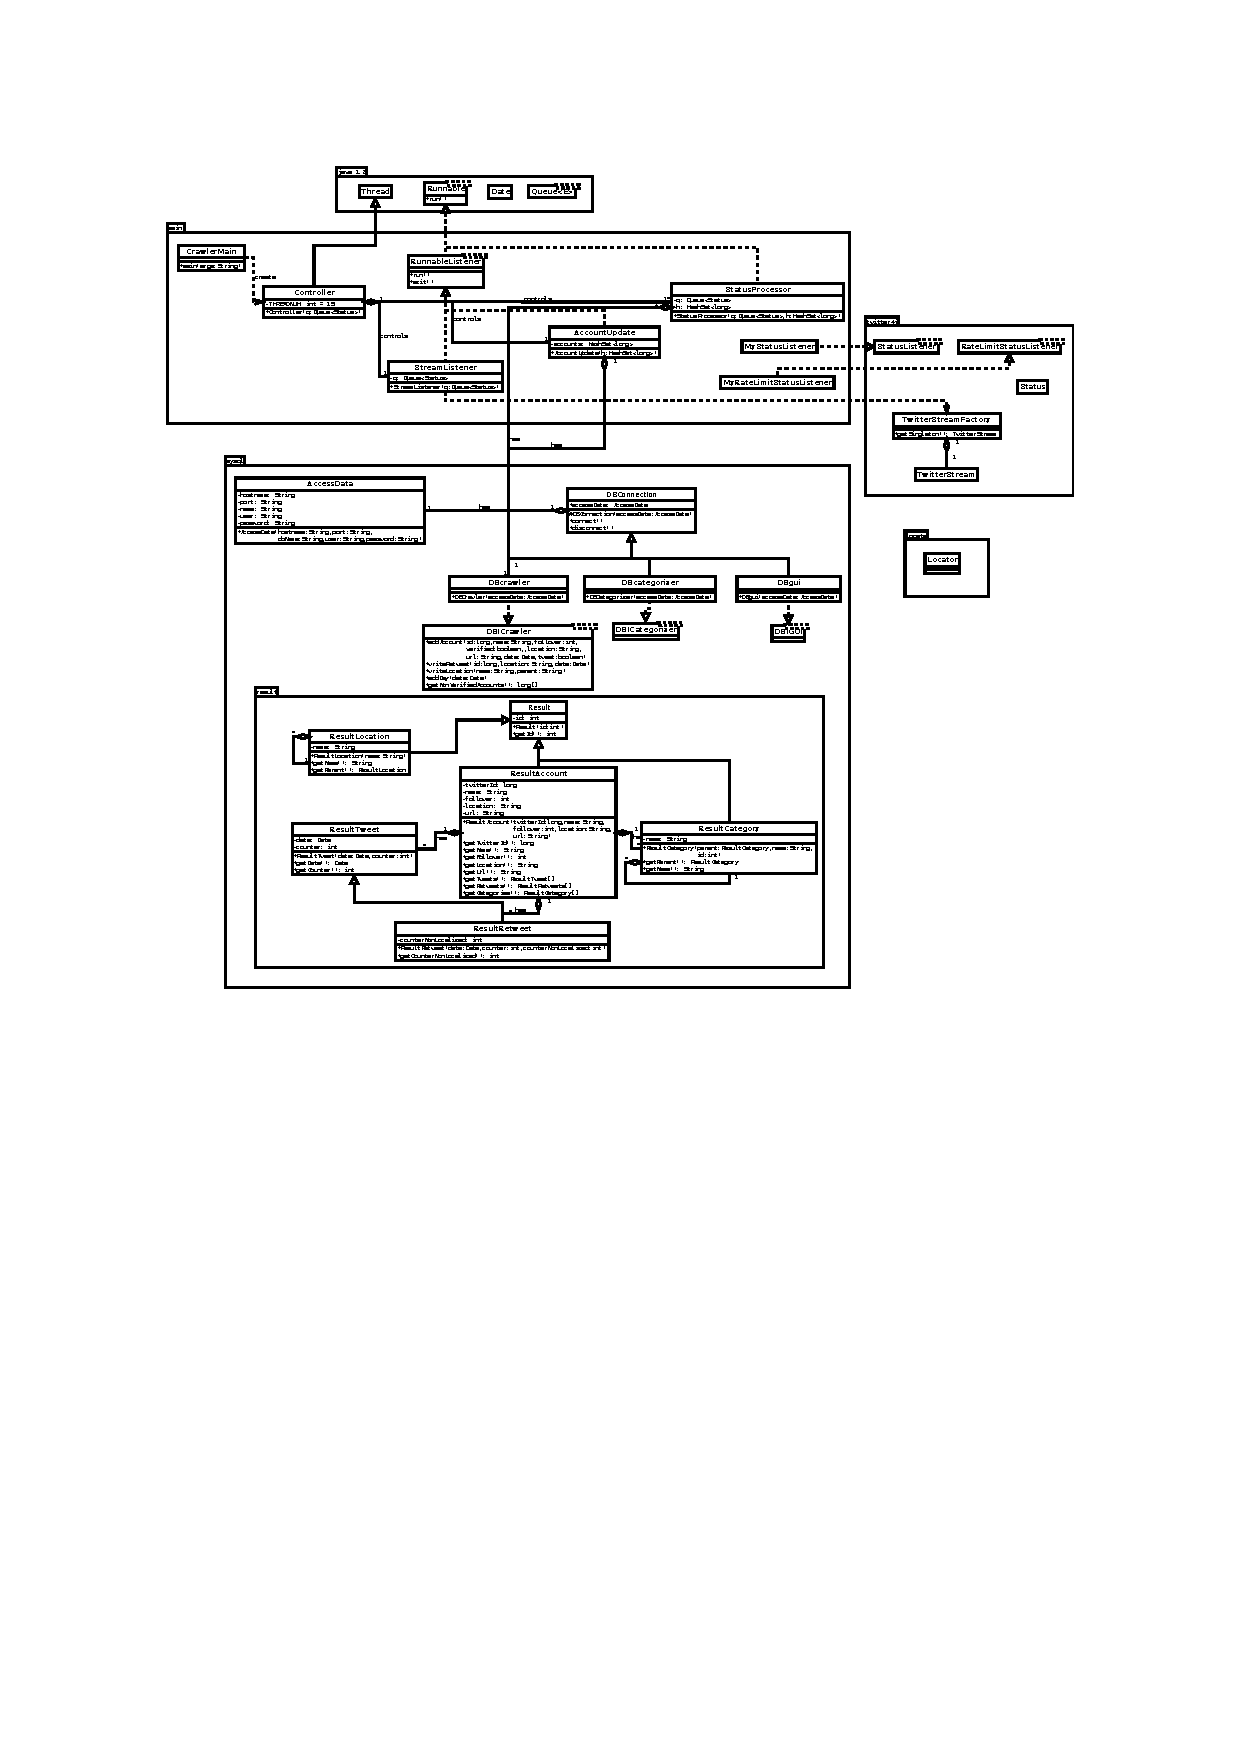
\includegraphics[width=\textheight,height=\textwidth,keepaspectratio=true,angle=-90]{dia/uml_crawler}
	\caption{UML-Klassendiagramm des Crawlers}
	\label{fig:uml_crawler}
\end{figure}

\begin{description}
\item[CrawlerMain] Klasse dient als Einstieg ins Programm. Sie überprüft die Eingabe für die Datenbankverbindung und startet einen Controller. Danach seht sie dem Benutzer über die Konsole zur Verfügung um das Programm zu überwachen.
\item[RunnableListener] Interface welches Runnable erweitert und zusätzlich noch eine exit-Methode fordert um Threads zu beenden.
\item[Controller] Diese Klasse koordiniert alle Aktionen die nötig sind um Daten bei Twitter abzuholen und in die Datenbank zu Schreiben. Dazu startet sie einen StreamListener, ein AccountUpdate und mehrere StatusProcessor's jeweils als Thread. Außerdem kontrolliert sie den Puffer und sorgt für ein sauberes Beenden des Programms indem alle Verbindungen ordnungsgemäß geschlossen und die Threads beendet werden.
\item[StreamListener] Stellt eine Verbindung zur Twitter-Streaming-API her und initialisiert einen MyStatusListener.
\item[AccountUpdate] Diese Klasse stellt eine Methode zur Verfügung um in der Datenbank periodisch nach Accounts zu suchen, welche manuell hinzugefügt wurden, aber auch wie Verifizierte behandelt werden sollen.
\item[StatusProcessor] Diese Klasse stellt die Funktionalität zur Filterung der Daten von Twitter zur Verfügung, welche sie aus dem Puffer nimmt. Außerdem bietet sie die Möglichkeit diese Daten in die Datenbank zu schreiben.
\item[MyStatusListener] Diese Klasse nimmt die Daten von Twitter entgegen und schreibt diese in einen Puffer.
\item[MyRateLimitStatusListener] Diese Klasse nimmt Meldungen von Twitter bezüglich RateLimits entgegen.
\item[Locator] Der Locator lokalisiert Accounts und Retweets mithilfe eines Webdienstes.
\end{description}

\section{Start des Crawlers}
Beim Starten des Crawlers werden sämtliche notwendigen Komponenten der Reihe nach gestartet. Dadurch wird garantiert, dass jede Komponente eine Umgebung vorfindet in der sie laufen kann und alle Ressourcen bereits zur Verfügung stehen. In \cref{fig:crawler_start} ist der Start des Crawlers beispielhaft mit 2 StatusProcessor's dargestellt.

\begin{figure}[h!]
	\centering
	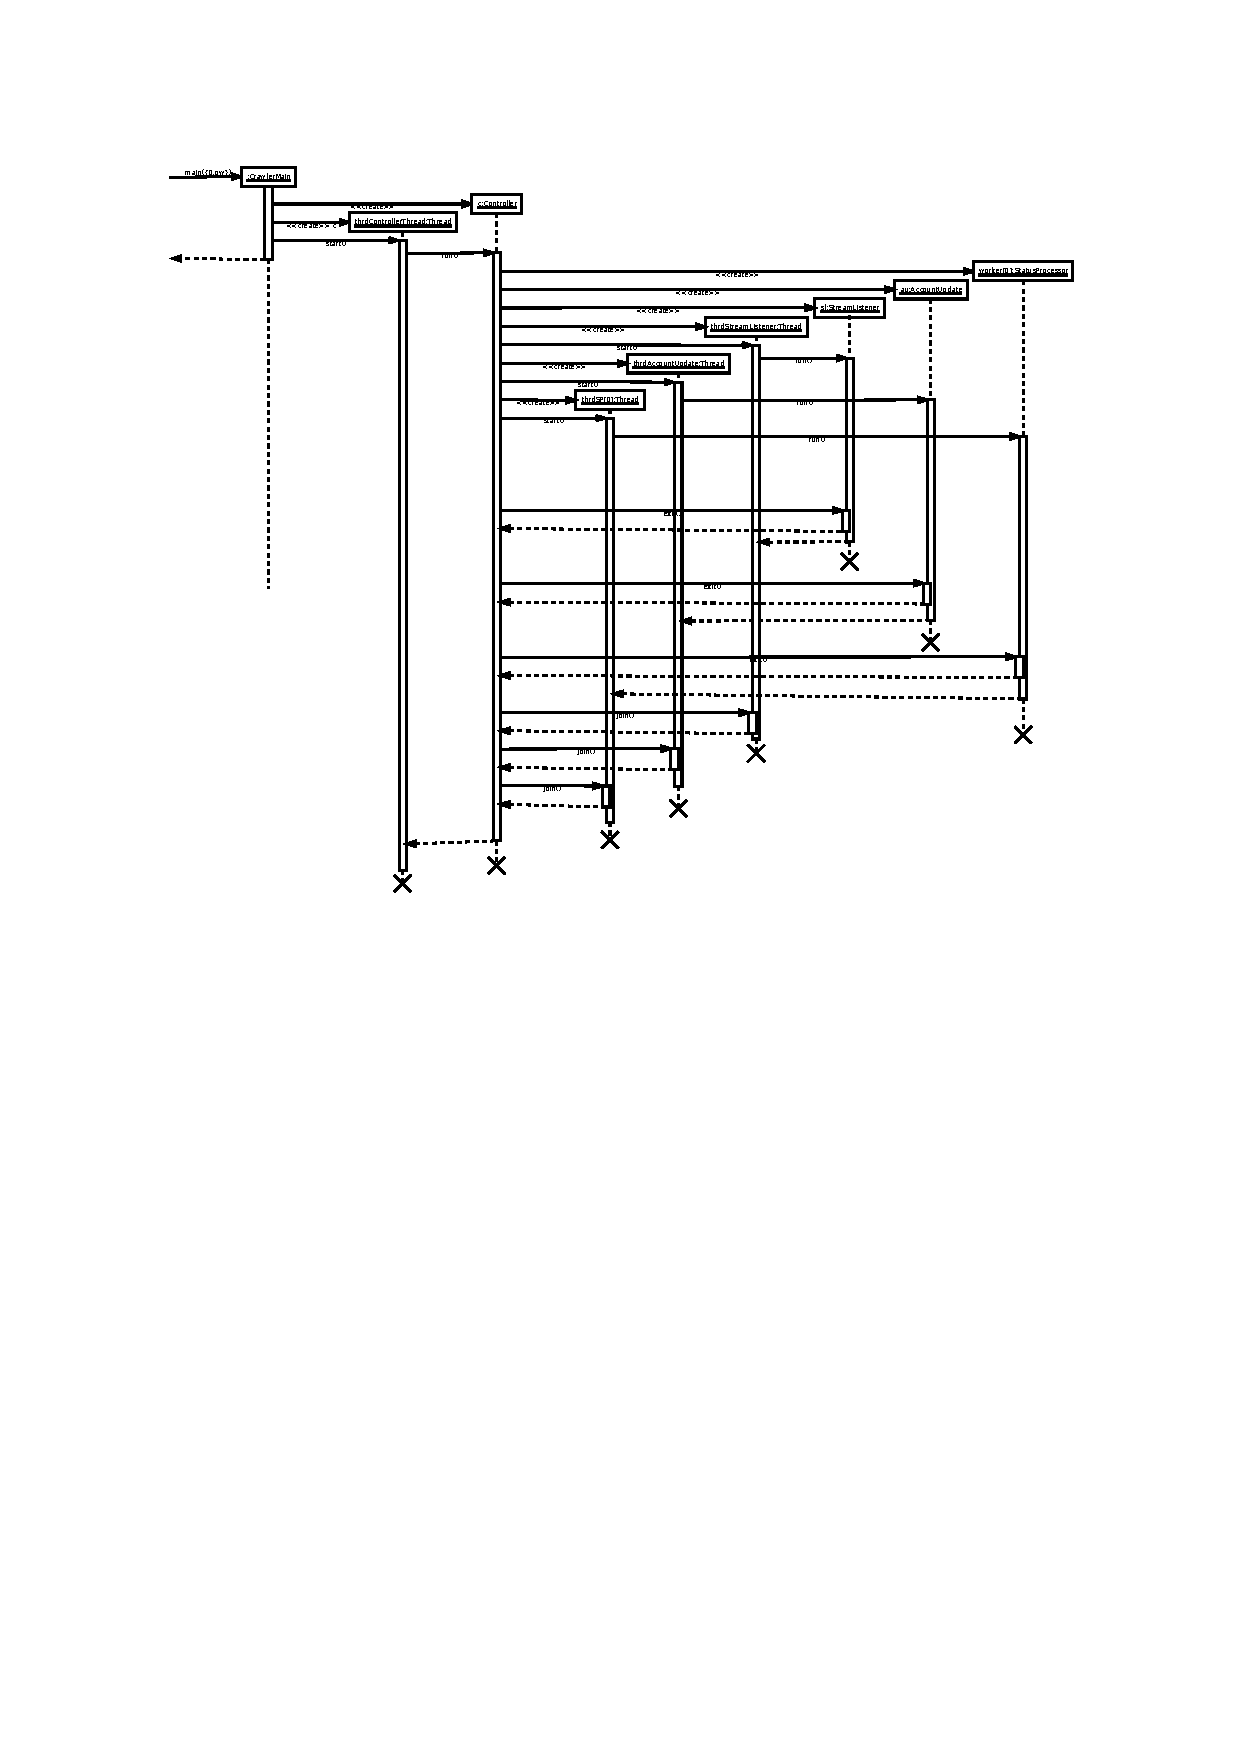
\includegraphics[width=\textheight,height=\textwidth,keepaspectratio=true,angle=-90]{dia/crawler_start_sequence}
	\caption{Sequenzdiagramm zum Start des Crawlers}
	\label{fig:crawler_start}
\end{figure}

\section{Verarbeitung der Daten von Twitter}
Um zu verdeutlichen wie die Daten von Twitter innerhalb des Crawlers verarbeitet werden, ist in \cref{fig:crawler_process} der Datenfluss durch den Crawler exemplarisch dargestellt. Dabei werden die Daten von Twitter abgeholt, gepuffert, dann gefiltert und schlussendlich in die Datenbank geschrieben.

\begin{figure}[h!]
	\centering
	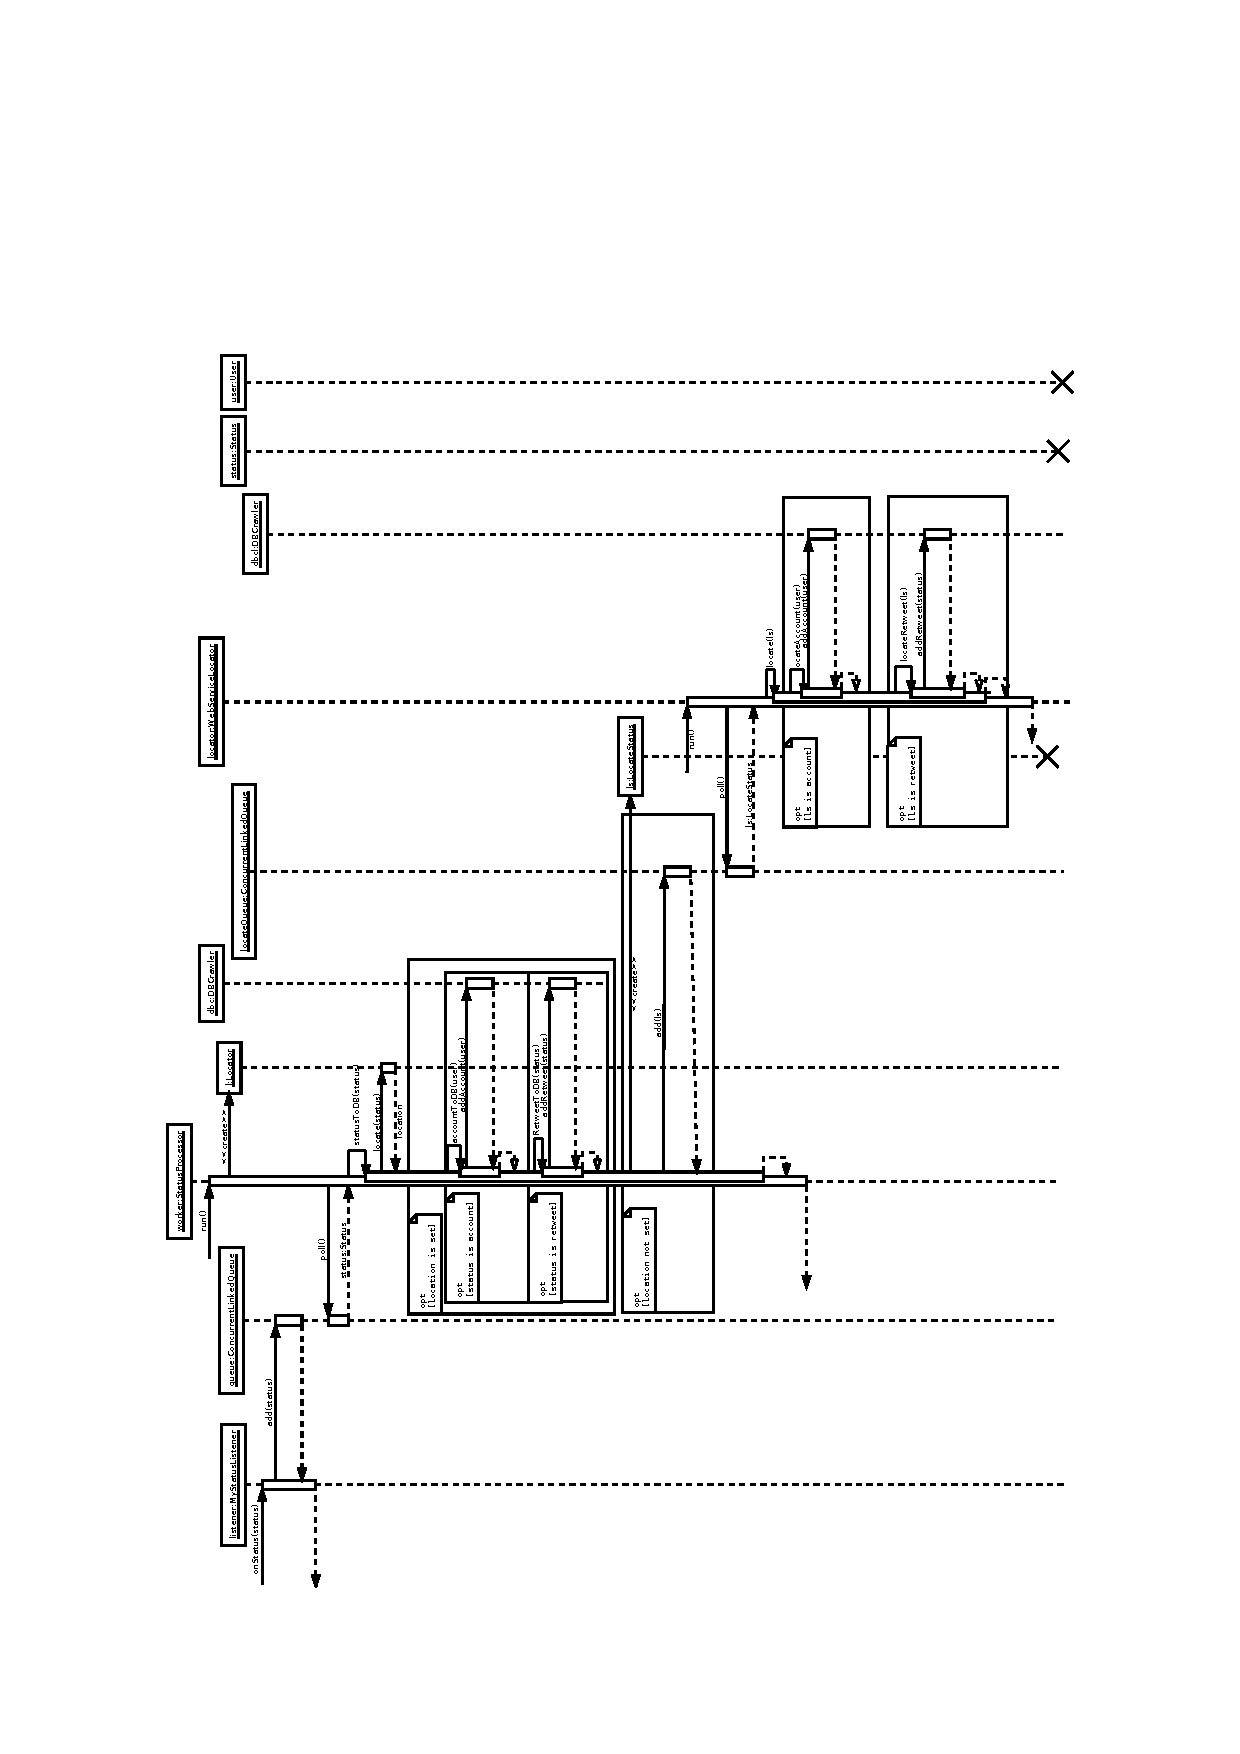
\includegraphics[width=\textheight,height=\textwidth,keepaspectratio=true,angle=-90]{dia/crawler_process_sequence}
	\caption{Sequenzdiagramm der Verarbeitung der Daten von Twitter}
	\label{fig:crawler_process}
\end{figure}